%Sie verstehen die Grundlagen eines OR-Mappers am Beispiel von Entity Framework Core
%Sie kennen die OR-Mapping-Konzepte in EF Core
%Sie kennen die Funktionalitäten der DbContext
%Sie können die CRUD-Operationen (inkl. LINQ) anwenden
%Sie können einfache Modelle erstellen und LINQ-Abfragen formulieren

\section{Entity Framework Core}
Unter .NET kommt ADO.NET als Entity Framework zum Einsatz. Man unterscheidet zwischen zwei Varianten wie die Entitätsklassen/Datenbanken erstellt werden können. Das Entity Framework muss mit NuGet installiert werden.
Es werden verschiedene Provider unterstützt: MS SQL, MySQL, PostgreSQL, SQLite, SQL Compact, in-memory.

\begin{description}
	\item[DB First] Man erstellt zuerst ein Domain Model und generiert daraus die Klassen. Man kann das Model auch von einer existierenden Datenbank ableiten und dann wieder die Klassen daraus generieren
	\item[Code First] Man erstellt die Model Klassen und lässt die Datenbank automatisch generieren.
	\item[Model First] Man erstellt zuerst das EDM (Entity Data Model) und generiert daraus die Database, sowie die Klassen
\end{description}




\subsection{OR-Mapping}
OR-Mapping ist eine Technik der Softwareentwicklung, mit der ein in einer objektorientierten Programmiersprache geschriebenes Anwendungsprogramm seine Objekte in einer relationalen Datenbank ablegen kann. EF Core verwendet für das verschiedene Provider, welche eine vielzahl von  SQL- und NoSQL-Datenbanken unterstützen.

\begin{figure}[h!]
  \center
  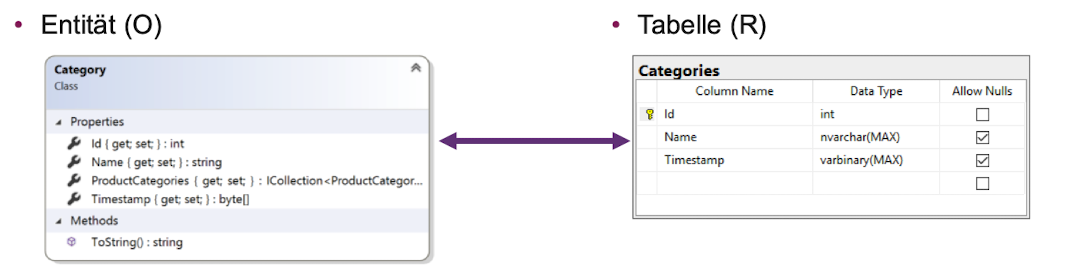
\includegraphics[width=0.75\linewidth]{OR-Mapping}
  \caption{Mapping von Objekten auf Relationen}
\end{figure}

\subsubsection{Mapping-Ansätze}
Das Mapping von Klassen auf das darunterliegende Speichermodell (Datenbank) kann auf drei verschiedene Ansätze realisiert werden. \textbf{Mapping: By Convention, By Attributes, By Fluent API}. 

\begin{minipage}{0,5\linewidth}
\begin{description}
    \item[Providers] Diverse relationale SQL Providers.
	\item[Entity] Ein Objekt mit einem Key (z.B ID). Mehrere dieser Objekte werden zu einem Entity-Set zusammengefasst.
	\item[Mapping] Mapping der Klassen auf das darunter liegende Speichermodell.
	\item[Mappingansätze] Zuordnung von Entity Type zu Storage Entity, Property zu Column, Entity Key zu Primary Key, Foreign Key zu Relationship.
	\item[Storage Entity] Relationales Modell/Graph/Collection, abhängig vom gewählten Provider. Ausprägungen: Table, View, Sotrec Procedures, etc. Inhalte: Columns, Primary KEys, Unique Key Constraints, Foreign Keys.
	\item[Association] Definiert eine Assotiation zwischen Entitäten (z.B Navigation Properties, Foreign Keys).
\end{description}

\end{minipage}
\begin{minipage}{0,5\linewidth}
	\center
  	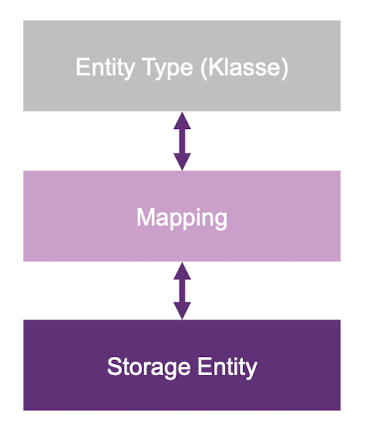
\includegraphics[width=0.5\linewidth]{or}	
\end{minipage}

\textbf{Mapping-Arten:} Das Mapping kann über das Entity-Level sowie das Attribut-Level realisiert werden.

\begin{minipage}{0,5\linewidth}
	\textbf{Entity-Level}\\
	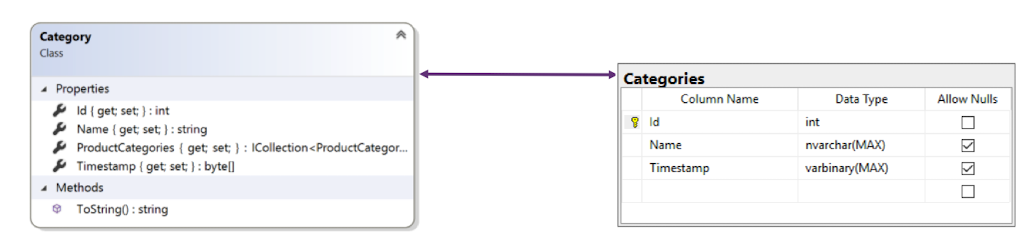
\includegraphics[width=\linewidth]{entity-level}
\end{minipage}
\begin{minipage}{0,5\linewidth}
	\textbf{Attribut-Level}\\
	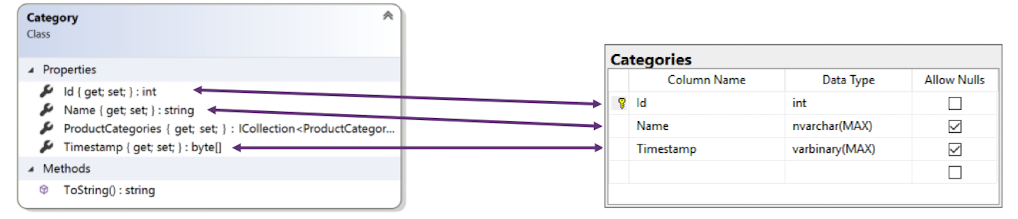
\includegraphics[width=\linewidth]{attribut-level}
\end{minipage}

\subsubsection{Model}
\begin{description}
    \item[Convention] Automatisches Mapping ohne explizite Konfiguration.
    \item[Fluent API] Extensions Method Syntax, Überschriebene Methode von ''OnModelCreating'' im DbContext \lstinline|protected override void OnModelCreating(ModelBuilder modelBuilder)|.
    \item[Data Annotations|Attributes] Deklaratives Mapping, Attribute direkt auf Model-Klassen
\end{description}

\textbf{Include/Exclude Entities}
\begin{lstlisting}
public class ShopContext : DbContext {
    // Convention - DbSet-Property im Context
    public DbSet<Category> Categories { get; set; }
    
    // Fluent API - Entry im Builder oder Ignore im Model Builder
    protected override void OnModelCreating( ModelBuilder modelBuilder) {
        modelBuilder.Entity<AuditEntry>();          
        modelBuilder.Ignore<Metadata>();
    }
}
public class Category {
    public int Id { get; set; }
    public string Name { get; set; }
    public ICollection<Product> Products { get; set; }  // Convention - Indirekt via Navigation Property
    public ICollection<Metadata> Metadata { get; set; }
}
public class Product { /* ... */ }
public class AuditEntry { /* ... */ }
[NotMapped]                               // Data Annotations
public class Metadata { /* ... */ }
\end{lstlisting}

\textbf{Include/Exclude Properties}
\begin{lstlisting}
public class ShopContext : DbContext {
    public DbSet<Category> Categories { get; set; }
    protected override void OnModelCreating(ModelBuilder modelBuilder) {
        modelBuilder.Entity<Category>()
            .Property(b => b.Name);                     
        modelBuilder.Entity<Category>()
            .Ignore(b => b.LoadedFromDatabase);  // Fluent API - Ignore im Builder
    }
}
public class Category {
    public int Id { get; set; }
    public string Name { get; set; }
    [NotMapped]                                               // Data Annotations
    public DateTime LoadedFromDatabase { get; set; }
}
\end{lstlisting}

\textbf{Keys}
\begin{lstlisting}
public class ShopContext : DbContext {
    public DbSet<Category> Categories { get; set; }
    protected override void OnModelCreating(ModelBuilder modelBuilder) {
        modelBuilder.Entity<Category>()
            .HasKey(e => e.Id)                              // Fluent API - Einzige Moeglichkeit fuer Composite Keys
            .IsRequired();
    }
}
public class Category {
    [Key]                                  // Data Annotations
    public int Id { get; set; }
    public string Name { get; set; }
}
public class Tanslation {
    public string Language { get; set; }
    public int CategoryId { get; set; }
}
\end{lstlisting}

\textbf{Required/Optional}
\begin{lstlisting}
public class ShopContext : DbContext {
    public DbSet<Category> Categories { get; set; }
    protected override void OnModelCreating(ModelBuilder modelBuilder) {
        modelBuilder.Entity<Category>()
            .Property(e => e.Name)
            .IsRequired();                // Fluent API
    }
}
public class Category {
    public int Id { get; set; }
    [Required]                             // Data Annotations
    public string Name { get; set; }
    public bool? IsActive { get; set; }
}
\end{lstlisting}

\textbf{Maximum Length}
Convention: Keine Restriktion / z.b. NVARCHAR(MAX), 450 Zeichen bei Keys
\begin{lstlisting}
.Property(e => e.Name).HasMaxLength(500)                 // Fluent API
[MaxLength(500)]                                         // Data Annotations
\end{lstlisting}

\textbf{Indexes} 
Convention: Werden bei Foreign Keys automatisch erstellt
\begin{lstlisting} 
modelBuilder.Entity<Category>()               // Fluent API - Non-unique Index
    .HasIndex(b => b.Name);
modelBuilder.Entity<Category>()               // Fluent API - Unique Index
    .HasIndex(b => b.Name)
    .IsUnique();
modelBuilder.Entity<Category>()               // Fluent API - Multi-column Index
    .HasIndex(b => new { b.Name, b.IsActive });
// Data Annotations - nicht unterstuetzt
\end{lstlisting}

\subsubsection{Relationale DB (SQL Server)}
\paragraph{Tabellen} Convention: Tabellenname = Klassenname (Pluralized) (z.b. dbo.Categories)
\begin{lstlisting}
// Fluent API - Name zwingend, Schema optional
modelBuilder.Entity<Category>()                         
    .ToTable("Category", schema: "dbo");
// Data Annotations - Name zwingend, Schema optional
[Table("Category", Schema = "dbo")]                     
public class Category {...}
\end{lstlisting}

\textbf{Spalten} 
Convention: Spaltenname = Property-Name
\begin{lstlisting}
// Fluent API
modelBuilder.Entity<Category>()                         
    .Property(e => e.Name)
    .HasColumnName("CategoryName", order: 1);
// Data Annotations
[Column("CategoryName", Order = 1)]                     
public string Name { get; set; }
\end{lstlisting}

\textbf{Datentypen / Default Values}
Convention: Keine Default Values
\begin{lstlisting}
// Fluent API
modelBuilder.Entity<Category>()                         
    .Property(e => e.Name)
    .HasColumnName("CategoryName")
    .HasColumnType("NVARCHAR(500)")                     // Datentyp-Name des Zielsystems
    .HasDefaultValue("---");                            // Default (Wert/Gueltige SQL Expression)
//Data Annotation - Datentyp-Name des Zielsystems, Default Values nicht unterstuetzt.
[Column("CategoryName", TypeName = "NVARCHAR(500)"] 
public string Name { get; set; }
\end{lstlisting}

\textbf{Relationship / Association – One-to-Many / Fully Defined Relationships} 
Convention: Collection Navigation Property (1-Ende), Reference Navigation Property (N-Ende), Foreign Key Property
\begin{lstlisting}
// Fluent API - HasOne/WithMany oder HasMany/WithOne
modelBuilder.Entity<Product>()
    .HasOne(p => p.Category)                            
    .WithMany(b => b.Products)
    .HasForeignKey(p => p.CategoryId)
    .HasConstraintName("FK_Product_CategoryId");
public class Product {
    public int Id { get; set; }
    public int CategoryId { get; set; }
    //Data Annotations - Auf Navigation Property wird Foreign Key Property definiert
    [ForeignKey(nameof(CategoryId))]                        
    public Category Category { get; set; }
}
public class Category {
    public int Id { get; set; }
    public ICollection<Product> Products { get; set; }
}
\end{lstlisting}

\textbf{Relationship / Association – One-to-Many / No Foreign Key Property} 
Convention: Collection Navigation Property (1-Ende), Reference Navigation Property (N-Ende)
\begin{lstlisting}
// Fluent API - .HasForeignKey weglassen
modelBuilder.Entity<Product>()
    .HasOne(p => p.Category)
    .WithMany(b => b.Products)                          
    .HasConstraintName("FK_Product_CategoryId");
public class Product {
    public int Id { get; set; }
    //Data-Annotation - Foreign Key weglassen
    public Category Category { get; set; }              
}
public class Category {
    public int Id { get; set; }
    public ICollection<Product> Products { get; set; }
}
\end{lstlisting}

\textbf{Relationship / Association – One-to-Many / Single Navigation Property} Convention: Collection Navigation Property (1-Ende)
\begin{lstlisting}
//Fluent API - .HasOne ist anders
modelBuilder.Entity<Product>()
    .HasOne<Category>()
    .WithMany(b => b.Products)
    .HasConstraintName("FK_Product_CategoryId");
public class Product {
    //Data Annotations - Foreign Key + Navigation Property weglassen
    public int Id { get; set; }                         
}
public class Category {
    public int Id { get; set; }
    public ICollection<Product> Products { get; set; }
}
\end{lstlisting}

\textbf{Relationship / Association - One-to-one / Many-to-many} One-to-one + Many-to-many

\textbf{One-to-one:} Nur Reference Navigation Property, keine Collection Navigation Property, \lstinline|.HasOne(...).WithOne(...)|

\textbf{Many-to-many:} aktuell nicht unterstützt, work-around (Assoziations-Klasse, zwei One-to-many Relationships)


\subsection{DB Context}
Der DBContext ist das Herzstück des Entity Frameworks. Er ist die Verbindung zwischen unseren Entitätsklassen und der Datenbank. Der DBContext ist verantwortlich für die Datenbankinteraktionen wie das Abfragen der Datenbank und das Laden der Daten in den Speicher als Entität. Er verfolgt auch die an der Entität vorgenommenen Änderungen und speichert die Änderungen in der Datenbank. Kombinert die Patterns: Repository, Unit of Work.

\begin{itemize}
	\item \textbf{Design Time:} Model definierern (OR-Mapping), Konfiguration, Database Migrations.
	\item \textbf{Run-Time:} Connections verwalten, CRUD Operationen, Change Tracking, Caching, Transaction Management.
\end{itemize}

\textbf{DBContext Lifecyle}
\begin{itemize}
	\item \textbf{Sollte nicht zu lange leben:} Limitierte Anzahl Connections im Client Connection Pool, Change-Tracking wird über die Zeit ineffizient.
	\item \textbf{Sollte nicht geshared werden:} Ist nicht thread-safe, Exception kann Instanz unbrauchbar machen.
\end{itemize}

\begin{lstlisting}
using (ShopContext context = new ShopContext()) {
    /* Context / Database Operations */
}
\end{lstlisting}

\subsubsection{Change Tracking}
Registriert alle Änderungen an getrackten Entities. Aktualisiert den Entity State. Agiert ohne die Datenbank und schreibt nur die Änderungen (Keine Live Checks).
\begin{itemize}
	\item Add() -> Added 
	\item Remove() -> Deleted
	\item Update() -> Modified
	\item Unchanged() -> Unchanged
	\item Not tracked -> Detached
\end{itemize}

\begin{lstlisting}
// New Record
Category cat = new Category { Name = "Laptops" };  // EntityState.Detached
context.Add(cat);                                  // EntityState.Added
context.SaveChanges();                             // EntityState.Unchanged
cat.Name = "Notebooks";                            // EntityState.Modified
context.SaveChanges();                             // EntityState.Unchanged
context.Remove(cat);                               // EntityState.Deleted
context.SaveChanges();                             // EntityState.Unchanged
\end{lstlisting}

\subsubsection{Ladestrategien (Lazy, Explizit, Eager Loading)}
Es wird standardmässig Lazy Loading verwendet. \\
\begin{description}
	\item[Lazy Loading] Assoziationen werden per se nicht geladen werden aber bei Zugriff auf Property automatisch nachgeladen. Collections werden komplett geladen. Passiert in separater Abfrage.
	Daten werden erst geladen, wenn sie referenziert werden. z.B erst wenn effektiv auf die Membervariable (Liste aus mehreren Items) zugegriffen wird. Für das Lazy Loading müssen die Methoden \lstinline|virtual| definiert werden. 
	\item[Eager Loading] Assoziationen werden per se nicht geladen. Include() Statement für einzelne Assoziationen. Passiert in der gleichen Abfrage per JOIN.
	\item[Explicit Loading] Assoziationen werden per se nicht geladen und werden explizit nachgeladen. Collections werden komplett geladen. Passiert in separater Abfrage.
	Even with lazy loading disabled it is still possible to lazily load related entities, but it must be done with an explicit call. To do so you use the Load method on the related entity’s entry
\end{description}

\begin{lstlisting}
Order order = context.Orders.First();
var customer = order.Customer; //customer is ''null''
var items = order.Items; //items is ''null''
\end{lstlisting}

\begin{lstlisting}
// lazy loading - zusaetzliche Ladelogik ausfuehren bei Zugriff auf Property
//Variante 1: Manuell - Auf Auto-Properties verzichten & Logik manuell implementieren
//Variante 2: Proxies 
public class Order {
    public int Id { get; set; }
    public virtual Customer Customer { get; set; }      // virtual wichtig
}
public class OrderProxy : Order {
    public virtual Customer Customer { /* ??? */ }      // virtual wichtig
}
Order order = context
    .Orders
    .First();
\end{lstlisting}

\begin{lstlisting}
// eager loading - mit .Include wird definiert was alles zusaetzlich ins RAM geladen werden soll
Order order = context
    .Orders
    .Include(o => o.Customer)                           // Eager Loading
    .Include(o => o.Items)
        .ThenInclude(oi => oi.Product)                  // Cascaded eager loading
    .First();
\end{lstlisting}

\begin{lstlisting}
// explicit loading - .Load() fuehrt dazu dass die Daten nachgeladen und in den Parent geladen werden D.h. es wird eine neue Query an die DB gemacht.
Order order = context
    .Orders
    .First();
context
    .Entry(order)
    .Reference(o => o.Customer)                         // Parents
    .Load();
context
    .Entry(order)
    .Collection(o => o.Items)                           // Collections
    .Query()
    .Where(oi => oi.QuantityOrdered > 1)
    .Load();
\end{lstlisting}

\subsection{LINQ to Entities}
Das EF führt keine LINQ queries aus! Das EF Core generiert Queries und die Datenbank führt diese dann aus.
\textbf{Einfaches Beispiel}
\begin{lstlisting} 
// DbContext instanzieren, DB Verbindung oeffnen, Cache/Change Tracker initialisieren.
using (ShopContext context = new ShopContext()) {          
    Category category = context                     // Abfrage mit LINQ (direkt)
        .Categories
        .Single(c => c.Id == 1);
        
    category.Name = $"{category.Name} / Changed";     // Daten aendern / speichern 
    context.SaveChanges();
    
    var categories = context.Categories;
    foreach (Category c in categories) { Console.WriteLine(c.Name); }       // Abfrage mit LINQ (deferred)
}     // Context schliessen - Cache invalidieren / Datenbank-Verbindung zurueck in Connection Pool
\end{lstlisting}

\subsubsection{CUD Operationen (Create, Update, Delete)}
DbContext agiert nach dem Unit of Work (UoW) pattern. Objekt wird beim Laden aus der
Datenbank automatisch der UoW registriert. Änderungen werden aufgezeichnet. Beim Speichern werden alle Änderungen in einer einzigen Transaktion geschrieben.

\textbf{Insert}
\begin{lstlisting}
using (ShopContext context = new ShopContext()) {
    Category cat = new Category { Name = "Notebooks" };
    // Add to Context (3 alternatives)
    // - Use .Add(...) to apply to whole graph
    // - Use .State when only for this entity
    context.Add(cat);
    context.Categories.Add(cat);
    context.Entry(cat).State = EntityState.Added;
    // Save  SQL is executed here
    context.SaveChanges();
    // Check Primary Key
    int id = cat.Id; // Category.Id is populated
}
\end{lstlisting}

\textbf{Update}
\begin{lstlisting}
using (ShopContext context = new ShopContext()); 
Category cat = await context
	.Categories 
	.FirstAsync();
// Change 
cat.Name = "Changed";

// Save  SQL is executed here 
await context.SaveChangesAsync();
\end{lstlisting}

\textbf{Delete}
\begin{lstlisting}
using (ShopContext context = new ShopContext()) {
    Category cat = context.Categories.First(c => c.Name == "Notebooks");
    // Remove (3 alternatives)
    // - Use .Remove(...) to apply to whole graph
    // - Use .State when only for this entity
    context.Remove(cat);
    context.Categories.Remove(cat);
    context.Entry(cat).State = EntityState.Deleted;
    // Save  SQL is executed here
    context.SaveChanges();              
}
\end{lstlisting}

\subsubsection{CUD von Assoziationen}
Assoziationen können durch drei Operationen angepasst werden: Anpassung Navigation Properties, Hinzufügen/Entgernen von Elementen in Collection Navigation Propeties, Setzen des Foreign keys.

\textbf{Durch Anpassung von Navigation Properties}\\
\lstinline{order.Customer = customer}

\textbf{Hinzufügen / Entfernen von Elementen in Collection Navigation Properties} \\
\begin{lstlisting}
customer.Orders.Add(order);
customer.Orders.Remove(order);
\end{lstlisting}

\textbf{Setzen des Foreign Keys} \\
\lstinline{order.CustomerId = 1;} \\
--> einzige Variante, welche keine weiteren Datenbankzugriffe benötigt

\textbf{Insert Object Graph} \\
\begin{lstlisting}
using(ShopContext context = new ShopContext()) {
    Customer cust = new Customer {
        Name = "Anna"
        Orders = new List<Order> {
            new Order { /* ... */ },
            new Order { /* ... */ }
        }
    };
    // Add to Context
    context.Add(cust);
    // Save - SQL is executed here
    context.SaveChanges();
}
\end{lstlisting}

\textbf{Insert Related Entity} \\
\begin{lstlisting}
using(ShopContext context = new ShopContext()) {
    Customer cust = context
        .Customers
        .Include(c => c.Orders)
        .First();
    cust.Orders.Add(new Order());
    
    // Save - SQL is executed here
    context.SaveChanges();
}
\end{lstlisting}

\textbf{Change Relationship 1} \\
\begin{lstlisting}
using(ShopContext context = new ShopContext()) {
    Order order = context
        .Orders
        .First();
    //Change - via Nav.Property
    order.Customer = context
        .Customers
        .First(c => c.Name == "Angela");
    
    // Save - SQL is executed here
    context.SaveChanges();
}
\end{lstlisting}

\textbf{Change Relationship 2} \\
\begin{lstlisting}
using(ShopContext context = new ShopContext()) {
    Order order = context
        .Orders
        .First();
    //Change - via Foreign Key
    order.CustomerId = 2;
    
    // Save - SQL is executed here
    context.SaveChanges();
}
\end{lstlisting}

\subsection{Optimistic Concurrency}
\textbf{Optimistic:} Transaktionen laufen unbehindert an. Beim Abschliessen wird in einer Validierungsphase überprüft, ob Konflikte aufgetreten sind und gegebenenfalls die Transaktion zurückgesetzt.

Wenn ein Objekt im gleichen Context geladen wird, gibt der Context das gecachte Objekt zurück. Die Objekte werden anhand ihrem Entity Key gecached.

\textbf{Erkennung von Konflikten:}
\begin{description}
  \item[Timestamp] Pro Record Timestamp / Row Version wird ein Timestamp erstellt. Beim Laden wird die Versionsnummer als Sessionzustand vermerkt. Validierung: Beim Zurückschreiben der Daten, wird die Session-Versionsnummer mit der Versionsnummer der DB verglichen.
  \item[Concurrency Token]  Für jedes geladene Datenfeld wird der ursprünglich gelesene Wert in der Applikation gespeichert. Änderungen werden auf einer Kopie ausgeführt. Validierung: Beim Zurückschreiben wird der ursprünglich gelesene Wert mit dem aktuellen Wert in der DB verglichen.
\end{description}

\textbf{Timestamp}
\begin{lstlisting}
public class ShopContext : DbContext {
    public DbSet<Category> Categories { get; set; }
    protected override void OnModelCreating(ModelBuilder modelBuilder) {
        modelBuilder.Entity<Category>()
            .Property(p => p.Timestamp)
            .IsRowVersion();    // Fluent API
    }
}
// --- ODER ---
[Timestamp]                     // Data Annotations
public byte[] Timestamp { get; set; }
\end{lstlisting}

\textbf{Concurrency Token} 
\begin{lstlisting}
public class ShopContext : DbContext {
    public DbSet<Product> Products { get; set; }
    protected override void OnModelCreating(ModelBuilder modelBuilder) {
        modelBuilder.Entity<Product>()
            .Property(p => p.Name)
            .IsConcurrencyToken();          // Fluent API
        modelBuilder.Entity<Product>()
            .Property(p => p.Price)
            .IsConcurrencyToken();          // Fluent API
    }
}
// --- ODER ---
[ConcurrencyCheck]              // Data Annotations
public string Name { get; set; }
\end{lstlisting}

\textbf{Konfliktbehandlung} \\
DbUpdateConcurrencyException beinhaltet fehlerhafte ”Entries” (Aktuelle Werte, Originale Werte, Datenbank Werte).

\begin{itemize}
	\item 1. Ignorieren - Der Fehler wird ignoriert und die Daten überschrieben
	\item 2. Benutzer Fragen - Der User entscheide, was passieren soll.
	\item 3. Autokorrektur - das Programm kann den Error verarbeiten
\end{itemize}

\subsection{Vererbung}
Wird aufgrund von: Speicherplatzverbrauchs, Zu vielen Tabellen, Inkonsistenzen nicht verwende. Es gibt drei verschiedene \textbf{Ansätze:} Table per Hierarchy, Table per Type, Table per Concrete Type. 

\textbf{Table per Hierarchy} \\
Eine Tabelle pro Vererbungs-Hierarchie (EF Core Standard). Nur über den DBContect definiertbar. Abgeleite Klassen als DbSet Properties definieren oder mit dem modebuilder.
\begin{lstlisting}
modelBuilder.Entity<Product>()
	.HasDiscriminator<int>("ProductType") 
	.HasValue<Product>(0) 
	.HasValue<MobilePhone>(1) 
	.HasValue<Tablet>(2);
\end{lstlisting}

\begin{figure}[h!]
  \center
  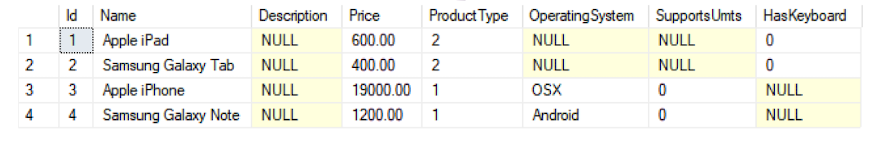
\includegraphics[width=0.75\linewidth]{tablehierarchy}
  \caption{Table per Hierarchy}
\end{figure}

\textbf{Table per Type} \\
Tabelle für jeden konkreten Typ mit allen benötigten Feldern. Keine Fremdschlüsselbeziehung (Parent-Child). Nachteil: Joins
\begin{itemize}
    \item \textbf{Tabelle "Products"}: Id, Name, Description, Price
    \item \textbf{Tabelle "MobilePhones"}: Id, OperatingSystem, SupportsUmts
    \item \textbf{Tabelle "Tablets"}: Id, HasKeyboard
\end{itemize}

\textbf{Table per Concrete Type} \\
Tabelle für Parent (gemeinsame Felder) und Tabellen für Childs (eigene Felder) mit Verweis auf Parent. Nachteil: Duplicate columns
\begin{itemize}
    \item \textbf{Tabelle "Products"}: Id, Name, Description, Price
    \item \textbf{Tabelle "MobilePhones"}: Id, Name, Description, Price, OperatingSystem, SupportsUmts
    \item \textbf{Tabelle "Tablets"}: Id, Name, Description, Price, HasKeyboard
\end{itemize}

\subsection{Database Migrations}
Während Entwicklung:
Modell anpassen, Migration erstellen, Review der Migration, eventuelle Korrekturen anbringen

Deployment:
Änderungen gemäss Migration-Reihenfolge auf Datenbank deployen, Rollback auf älteren Stand via Down-Migration möglich

\textbf{Migration erstellen}
\lstinline{dotnet ef migrations add InitialCreate}
-> DB wude noch nicht erstellt

\textbf{Datenbank Deployment}
\lstinline{dotnet ef database update}
-> DB wurde erstellt

\begin{lstlisting}
using(var context = new AngProjContext()) {
    var database = context.Database;
    //"Dev" Ansatz (loeschen / neu erstellen)
    database.EnsureDeleted(); //Loescht DB
    database.EnsureCreated(); //Erstellt DB falls nicht vorhanden
    
    //Automatische Migration auf neuesten Stand
    database.Migrate(); //Migration DB zur neusten Version
    
    //Migrations abfragen
    IEnumerable<string> migrations;
    migrations = database.GetMigrations(); //Abfrage von Migration-Names im DbContext
    migrations = database.GetPendingMigrations();
    migrations = database.GetAppliedMigrations();
    var m = context.GetService<IMigrator>(); 
    m.Migrate("<MigrationName>"); //Explizite Migration auf spezifische Version
}
\end{lstlisting}


\pagebreak